\documentclass{report}

% \usepackage[ngerman]{babel}
\usepackage[utf8]{inputenc}

% fonts
\usepackage{geometry,amsmath,amsfonts,metalogo,hyperref,mdwlist,array,multicol,fontawesome,color}
\usepackage[default,osf]{sourcesanspro}
\usepackage[scaled=.95]{sourcecodepro}
\linespread{1.3}

% captions and figures
\usepackage[font=small,labelfont=bf]{caption}
\usepackage{graphicx, subcaption, float}
\restylefloat{figure}

\usepackage{wrapfig}            % for floating images
\usepackage[export]{adjustbox}  % for frames

\begin{document}


%
%   SHOW OFF
%


{\centering

  \begin{figure}
    \vspace{3cm}

    \centering
    
\includegraphics[width=0.3\textwidth]{src/yield}

    \vspace{4cm}
  \end{figure}


  {\Huge\textbf{Yield Sign Detection}}
  \vspace{.4cm}

  Felix Hamann

  \vspace{.2cm}

  \today

}


%
%   CONTENT
%

\tableofcontents


\chapter{Introduction}

This document describes the implementation of a system to detect yield
signs from images. {\color{red}{To be written: Some general
    introduction (problem description, scope, constraints, reason)}}

\section{Requirements}

The system should be able to detect yield signs from the perspective
of a car participating in traffic. This means that the point of view
is approximately between one and two meters from the ground on the
right lane\footnote{Except for countries with left hand traffic that
  are not considered here.} of a street. There are no hard
requirements regarding size and quality of the images. For testing
purposes both small images with inferior quality and high resolution
images should be tested. This is necessary to make a prediction
whether the system is suitable for real-time use in videos. Videos may
be cropped and shrunk to fit these requirements. The detection should
work with changing ambient light. Without white balancing, the
standardized red color value of yield signs changes when captured by
camera based on the daytime. The color also varies greatly when the
sunlight is reflected on the sign.


\section{Notation}

All images are either two or three dimensional. Two dimensional images
are either grayscale or binary images, three dimensional images are
color images with three color components: red, green and blue (in this
order). Origin of each image is the top left corner and iteration is
row-major. This is reflected when addressing single pixel
values. Given some image \( I \), then \( I(y, x) \) returns the pixel
\( y \) in the images' vertical and \( x \) in the images' horizontal
direction. Binary images are two dimensional and every value is in
\(\{ 0, 1 \}\). Thus, boolean operations can be applied. Pixel values
of 0 are called ``black'' or ``false'' and values of 1 are called
``white'' or ``true''. Each step in the pipeline that is described in
chapter \ref{chap:pipeline} has a \( source \) image which is the
result of the previous step of the pipeline and a \( target \) image
that is written to.

{\color{red}{To do: Nice picture of the final result}}


\pagebreak
\chapter{The pipeline}
\label{chap:pipeline}

For yield sign detection a modular system of components is used. Each
step of the pipeline takes at least the result of the previous step as
input for processing. Simply put, color images are fed into the
pipeline and a set of yield sign descriptions is returned. Each
element of this set contains all three vertices and the center of the
sign.

\begin{figure}
  \centering
    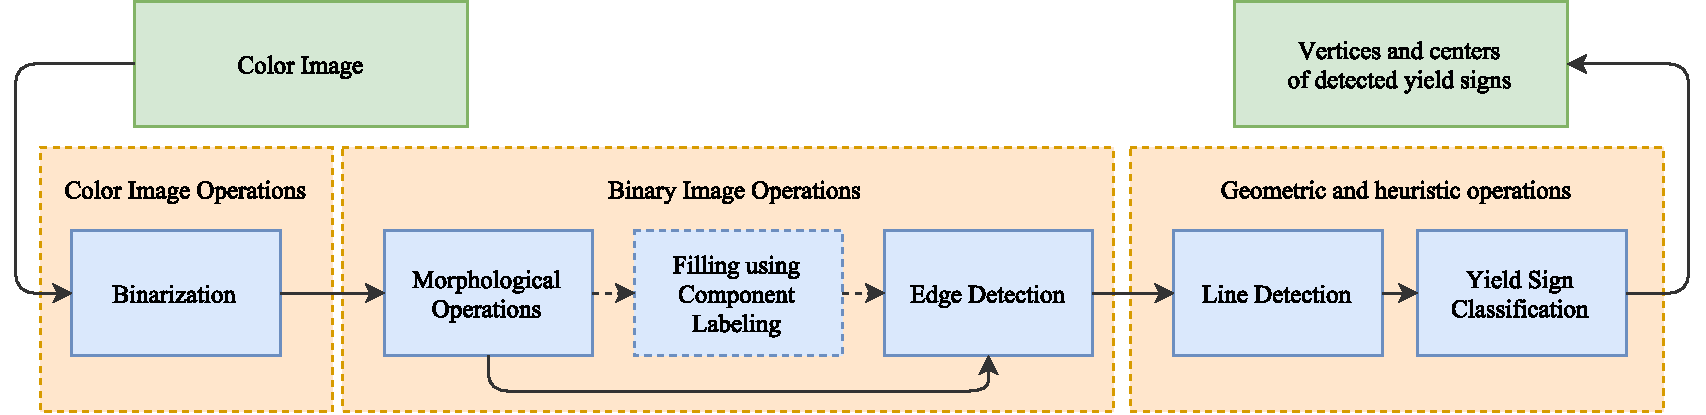
\includegraphics[width=1\textwidth]{src/pipeline}
  \caption{A high level overview of the processing pipeline}
  \label{img:pipeline}
\end{figure}

The pipeline itself consists of the following components: First the
red color component of the image is extracted. A threshold is
introduced to create a binary image masking all red areas. This is
described in section \ref{sec:pipeline_binarization}. The next
component applies morphological operations to enhance the quality of
the extracted areas. A description of this can be found in section
\ref{sec:pipeline_morph}. The following section
\ref{sec:pipeline_complab} describes how the amount of relevant red
areas can be greatly reduced by filling the ``background'' of the
image utilizing component labeling. As this proved quite useful but
hindered detection completely for some corner cases, this step can be
enabled optionally. The now remaining relevant areas are transformed
in such way that their shapes are defined by their edges
{\color{red}{(either dilation + xor or sobel)}}. Section
\ref{sec:pipeline_edgedet} describes this and the succeeding section
\ref{sec:pipeline_linedet} explains how this information can be used
to detect and extract lines from the image. After all lines are
extracted section \ref{sec:pipeline_yielddet} discusses how some
heuristics are applied to determine all relevant triangles and
classify whether those triangles could be yield signs. A graphical
depiction of this process is given in \ref{img:pipeline}.

{\color{red}{To do: Apply a median filter before or after
    segmentation?}}


\section{Segmentation}
\label{sec:pipeline_binarization}

The first step of the whole pipeline consists of extracting the red
color from the colored input image \textit{source}. Thus a mapping for
each pixel from three dimensions to one dimension is needed. Simply
returning the red color component does not suffice, as with larger
values of the green and blue components the source color either shifts
towards yellow, magenta or white. The method used in this application
takes a predefined red color vector, calculates the distance between
the currently considered pixel value and applies a threshold for
binarization to the target image. Equation \ref{eq:segmentation}
describes this mapping formally. Let \( \Gamma = \{0, 1, ..., 255\} \)
be all possible pixel values, \( v_{ref} \in \Gamma^3 \) the reference
color and \( \delta \in \mathbb{N} \) the threshold, then the pixel
value written to \( target \) depends on whether the threshold
undercuts the Frobenius norm.

\begin{equation}\label{eq:segmentation}
  \begin{split}
    norm & : \Gamma^3 \to \mathbb{R} \\
    norm(v, w) & = \sqrt{\sum_{1 \leq i \leq 3}(v_i - w_i)^2}  \\
    target(y, x) & =
    \begin{cases}
      1 & \quad \text{if } norm(source(y, x), v_{ref}) < \delta \\
      0 & \quad \text{else}
    \end{cases}
  \end{split}
\end{equation}

\begin{figure}
  \begin{subfigure}[t]{0.5\textwidth}
    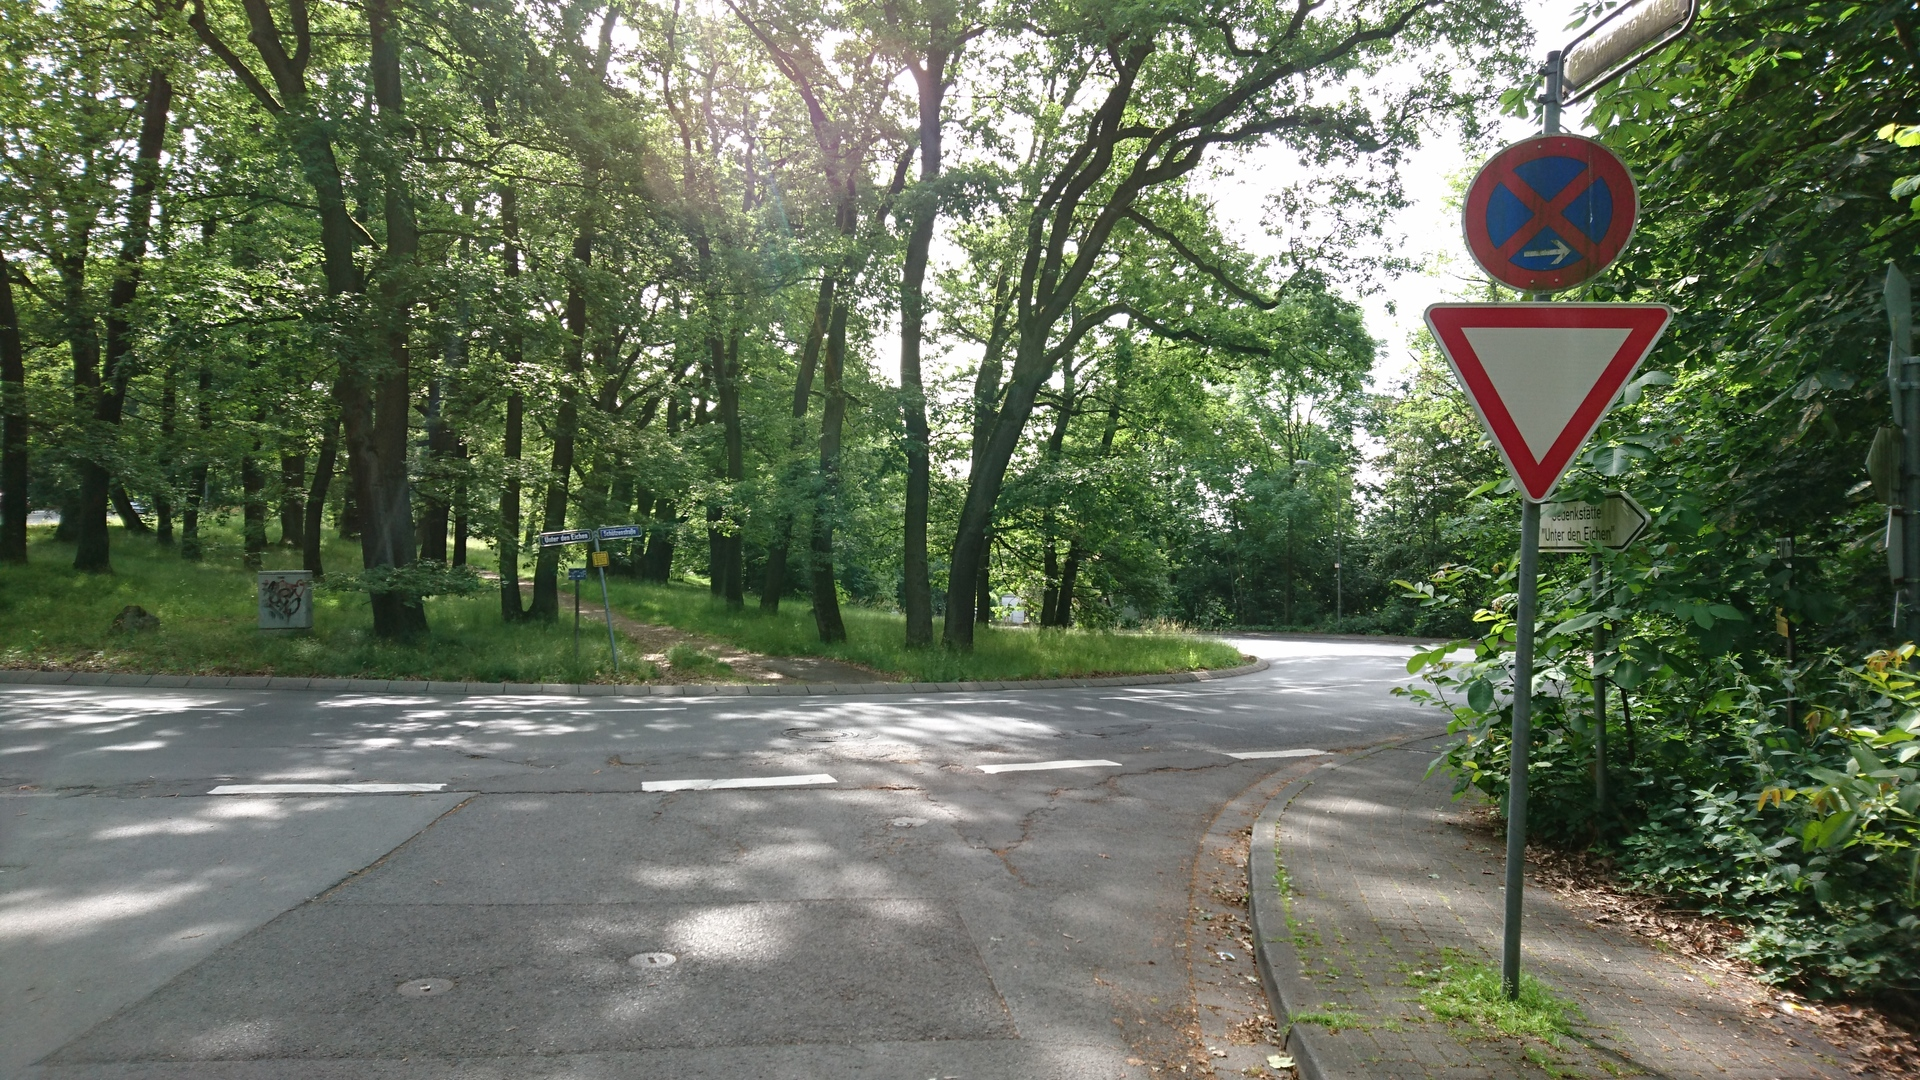
\includegraphics[width=1\textwidth]{src/segmentation/original}
  \end{subfigure}
  \quad
  \begin{subfigure}[t]{0.5\textwidth}
    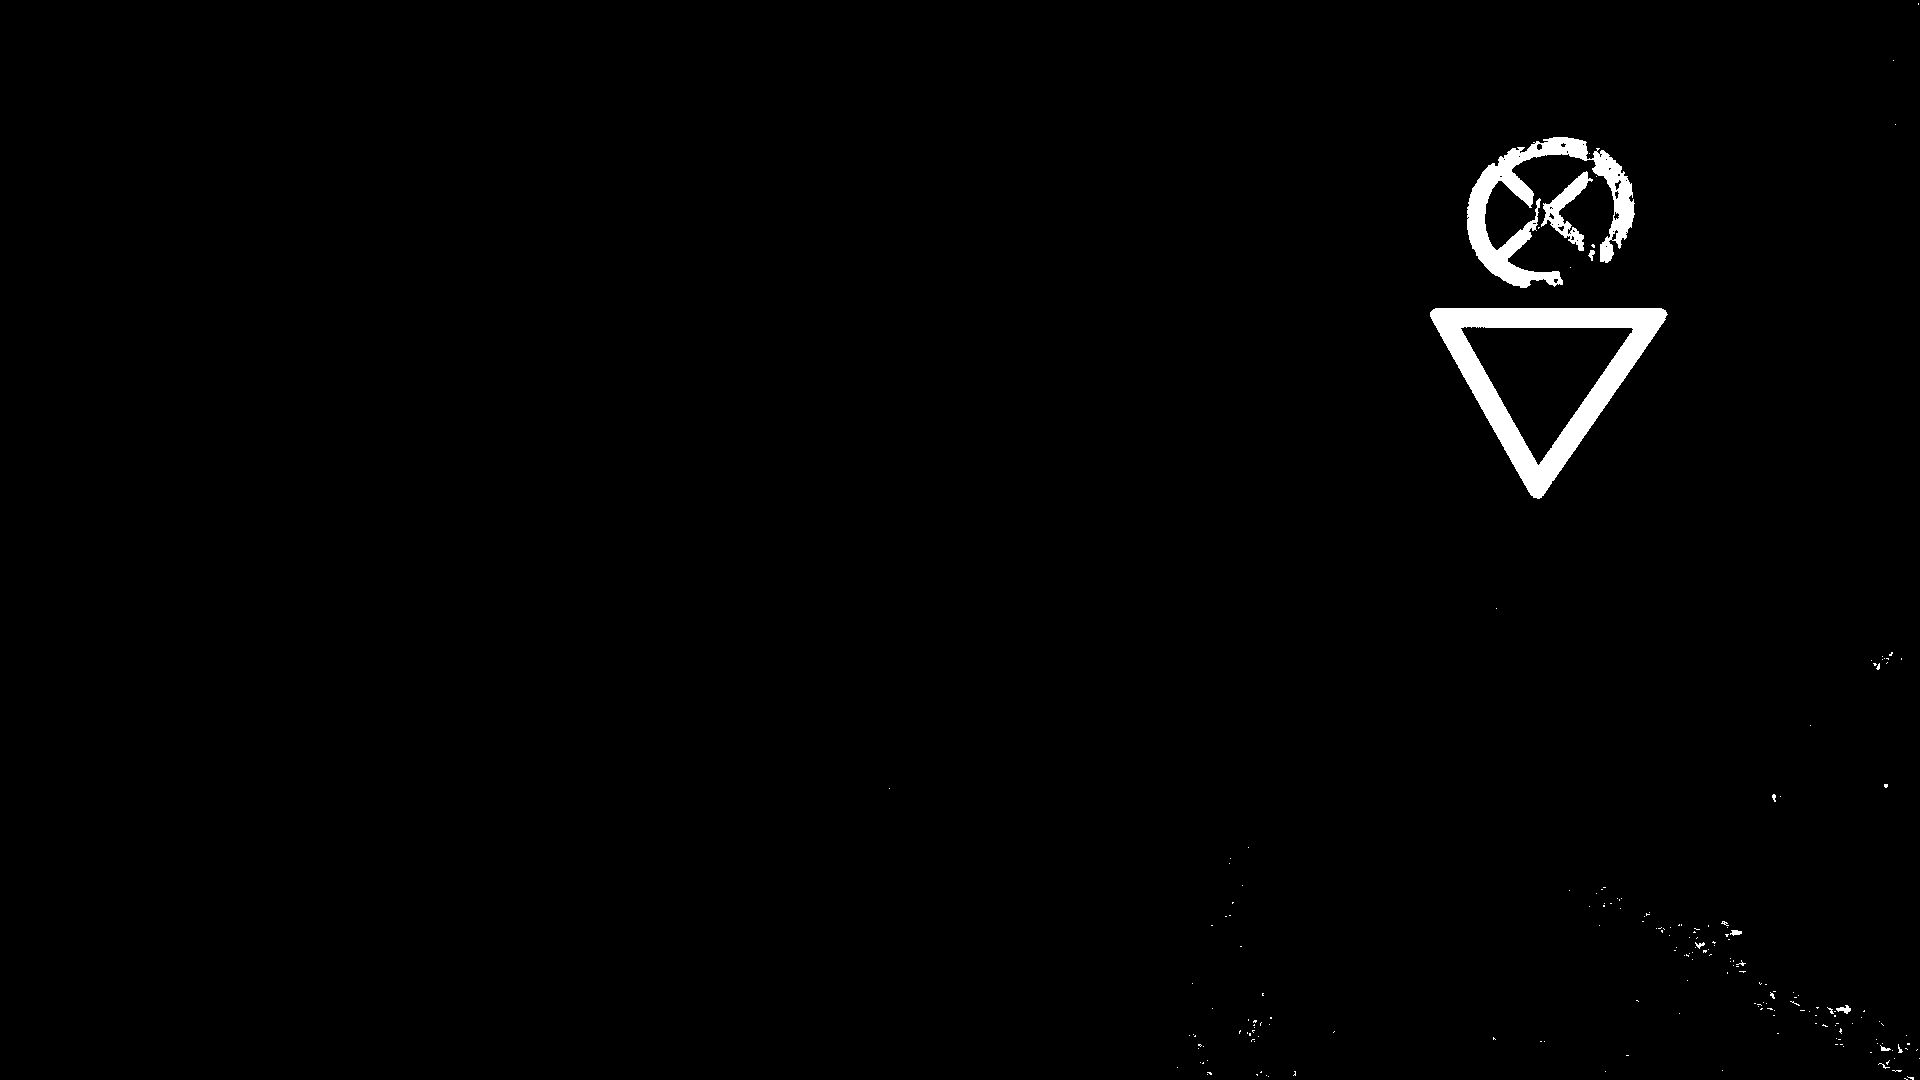
\includegraphics[width=1\textwidth]{src/segmentation/segmented}
  \end{subfigure}
  \caption{Color segmentation to create a binary image with red areas
    marked true. \\ Used parameters are \( v_{ref} = (180, 20, 20) \)
    and \( \delta = 100 \).}
\end{figure}


\section{Morphological operations}
\label{sec:pipeline_morph}

At this point of the pipeline, the \textit{source} image is a binary
image with all areas considered red marked true. The quality of the
image and found red areas depends greatly on a variety of factors. For
one the camera itself might introduce pixel errors to the picture,
resulting in falsely colored pixels (when the sensor is of inferior
quality or getting old) or blacked out areas (e.g. when the lens is
dirty). On the other hand the to-be-detected yield sign could be
dirty, altered by vandalism or simply reflect light which would
obscure its shape. As it is essential to expose the signs form for
best detection, some morphological operations may be applied for noise
removal.

The system implements two morphological operations that are separately
adjustable. These operations are called dilation and erosion. This is
called ``closing'' when combined. The purpose and functioning of these
algorithms are described below.


\subsection{Erosion and Dilation}

Main purpose of erosion is to remove white noise from the binary
image. For every pixel of the \textit{source} image, some range around
the pixel is considered. This range - as used the current
implementation - can be seen in \ref{eq:morph_mask} and is commonly
called ``structuring element'' \textit{S}. Now, for every pixel in the
\textit{source} image, the mask is applied and the target pixel is set
based on \ref{eq:morph_erosion}. Commonly speaking, the target pixel
is only set if all surrounding pixels masked by \textit{S} are also
set.

\begin{equation}\label{eq:morph_mask}
  S_{y, x} = \begin{bmatrix}

    -              & source(y-1, x) & -              \\
    source(y, x-1) & source(y, x)   & source(y, x+1) \\
    -              & source(y+1, x) & -

  \end{bmatrix}
\end{equation}

\begin{equation}\label{eq:morph_erosion}
  target(y, x) = 1 \iff \bigwedge_{s \in S_{y, x}} s \neq 0
\end{equation}

The functioning of the algorithm is depicted in
\ref{eq:morph_erosion-example}. Closed white components shrink by the
factor determined by the size of \textit{S}. Spurious grains of white
are eliminated completely. Thus the erosion is used to remove white
noise on black backgrounds such as the grain on the bottom right of
the example.

\begin{align}\label{eq:morph_erosion-example}
  source = \begin{bmatrix}
    0 & 0 & 0 & 0 & 0 & 0 \\
    0 & 1 & 1 & 1 & 1 & 0 \\
    0 & 1 & 1 & 1 & 1 & 0 \\
    0 & 1 & 1 & 1 & 1 & 0 \\
    0 & 1 & 1 & 1 & 1 & 0 \\
    0 & 0 & 0 & 0 & 0 & 1
  \end{bmatrix}
  & &
  \mapsto
  & &
  target = \begin{bmatrix}
    0 & 0 & 0 & 0 & 0 & 0 \\
    0 & 0 & 0 & 0 & 0 & 0 \\
    0 & 0 & 1 & 1 & 0 & 0 \\
    0 & 0 & 1 & 1 & 0 & 0 \\
    0 & 0 & 0 & 0 & 0 & 0 \\
    0 & 0 & 0 & 0 & 0 & 0
  \end{bmatrix}
\end{align}

The dilation operation alters the image in such way that closed white
forms expand by the factor determined by \textit{S}. Grains of black
are removed from white backgrounds. The algorithm itself works
analogous to the erosion algorithm but pixels in the target image are
set if any of the masked source pixels is white. The equation changes
accordingly and is defined in \ref{eq:morph_dilation}. An example is
given in \ref{eq:morph_dilation-example}. It can be observed that the
white form grows and the black grains inside that form vanish. Note
that the form is not smoothed and the cut propagates to the target.

\begin{equation}\label{eq:morph_dilation}
  target(y, x) = 1 \iff \bigvee_{s \in S_{y, x}} s \neq 0
\end{equation}

\begin{align}\label{eq:morph_dilation-example}
  source = \begin{bmatrix}
    0 & 0 & 0 & 0 & 0 & 0 \\
    0 & 0 & 0 & 0 & 0 & 0 \\
    0 & 1 & 0 & 1 & 1 & 0 \\
    0 & 1 & 1 & 1 & 1 & 0 \\
    0 & 1 & 1 & 0 & 1 & 0 \\
    0 & 1 & 1 & 1 & 1 & 0
  \end{bmatrix}
  & &
  \mapsto
  & &
  target = \begin{bmatrix}
    0 & 0 & 0 & 0 & 0 & 0 \\
    0 & 1 & 0 & 1 & 1 & 0 \\
    1 & 1 & 1 & 1 & 1 & 1 \\
    1 & 1 & 1 & 1 & 1 & 1 \\
    1 & 1 & 1 & 1 & 1 & 1 \\
    1 & 1 & 1 & 1 & 1 & 1
  \end{bmatrix}
\end{align}


\subsection{Opening and closing}

When erosion and dilation are combined they form an operation called
opening. This is due to the fact that if any forms are connected by
thinner areas this connection vanishes through erosion and the
original forms size is restored by dilating again afterwards. The
opposite effect occurs when first dilating and then eroding the
image. Here, thin connections are strengthened and connections between
forms may be established. This proves useful if a closed yield sign
shapes are required even if somebody took a pencil and drew over the
red area or light reflections break the red surface. The number of
iterations are free parameters of the system and may be
adjusted. Introducing another erosion step to remove white noise
mostly resulted in eroding the yield sign itself and is therefore no
longer part of the pipeline.

\begin{figure}
  \begin{subfigure}[t]{0.5\textwidth}
    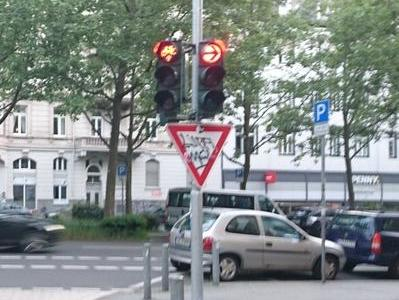
\includegraphics[width=1\textwidth]{src/closing_0}
    \subcaption{Original image}
  \end{subfigure}
  \quad
  \begin{subfigure}[t]{0.5\textwidth}
    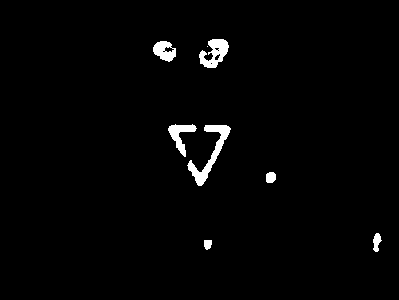
\includegraphics[width=1\textwidth]{src/closing_1}
    \subcaption{Segmented image}
  \end{subfigure}
  \begin{subfigure}[t]{0.5\textwidth}
    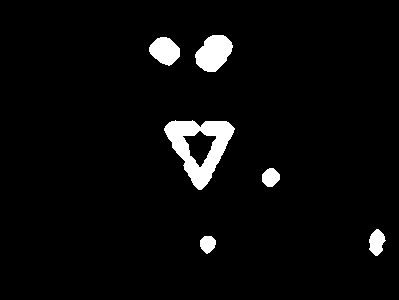
\includegraphics[width=1\textwidth]{src/closing_2}
    \subcaption{After dilation}
  \end{subfigure}
  \quad
  \begin{subfigure}[t]{0.5\textwidth}
    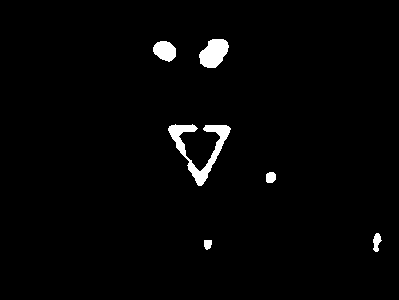
\includegraphics[width=1\textwidth]{src/closing_3}
    \subcaption{After erosion}
    \label{subcap:erosion}
  \end{subfigure}
  \caption{Closing applied to an image with a vandalized yield
    sign. Note how the form is closed in \ref{subcap:erosion} on the
    left side. However, the number of iterations were not sufficient
    to close the form completely. All noise is removed from the red
    lights.}
\end{figure}


\section{Component labeling}
\label{sec:pipeline_complab}

This optional step tries to greatly reduce the impact of red image
areas that are not yield signs. The basic idea is that yield signs
enclose a white triangle and thus there are black areas enclosed by
closed white borders in the binary image. If all black areas are
labeled, the label with the most associated pixels must be the
background - assuming the yield sign is not the most prominent object
captured. All forms that do not enclose any area vanish that way,
greatly reducing the amount of considered objects. Because the
algorithm is defined for labeling white areas, the source image needs
to be inverted first.

The algorithm works by iterating the image from top-left, selecting
all white pixels and checking whether a new label needs to be
introduced or - if the neighbors are already labeled adopt that label
for the current pixel. Formally, given a mask \textit{M} and a set \(
L = \{1, 2, ... \} \) of unassigned labels, the target pixels value is
given by formula \ref{eq:label}. Because multiple values can be
returned by \textit{M}, another set \textit{E} is needed to store all
equivalents. After the first labeling step, the equivalents are
resolved by assigning the smallest label of possible candidates. This
algorithm is called two-pass algorithm and the form of \textit{L}
checks for 8-connectivity as all eight neighboring pixels are taken
into account.

\begin{equation}
  M_{y, x} = \begin{bmatrix}
    source(y-1, x-1) & source(y-1, x) & source(y-1, x+1) \\
    source(y, x-1)   & source(y, x)   & -
  \end{bmatrix}
\end{equation}


\begin{equation}\label{eq:label}
    target(y, x) =
    \begin{cases}
      min(L) \quad L = L \setminus l & \quad \text{if } \forall m \in M_{y, x}: m = 0 \\
      any(M) \quad E = E \cup \{(m, n)\} \quad m, n \in M_{y, x} & \quad \text{else}
    \end{cases}
\end{equation}

After labeling all distinct components of the image, the component
with the largest amount of associated pixels is set to white and the
image is again reversed. Although this step proves to be very
effective it has one big drawback: As soon as the detected yield sign
shape is not closed the whole detection system fails immediately. This
does not happen otherwise as even without a closed form, the other
edges are prominent enough to allow detection. Thus this step can
optionally be enabled or disabled. An example where this step proves
quite useful can be found in figure \ref{img:filling}

\begin{figure}
  \centering
    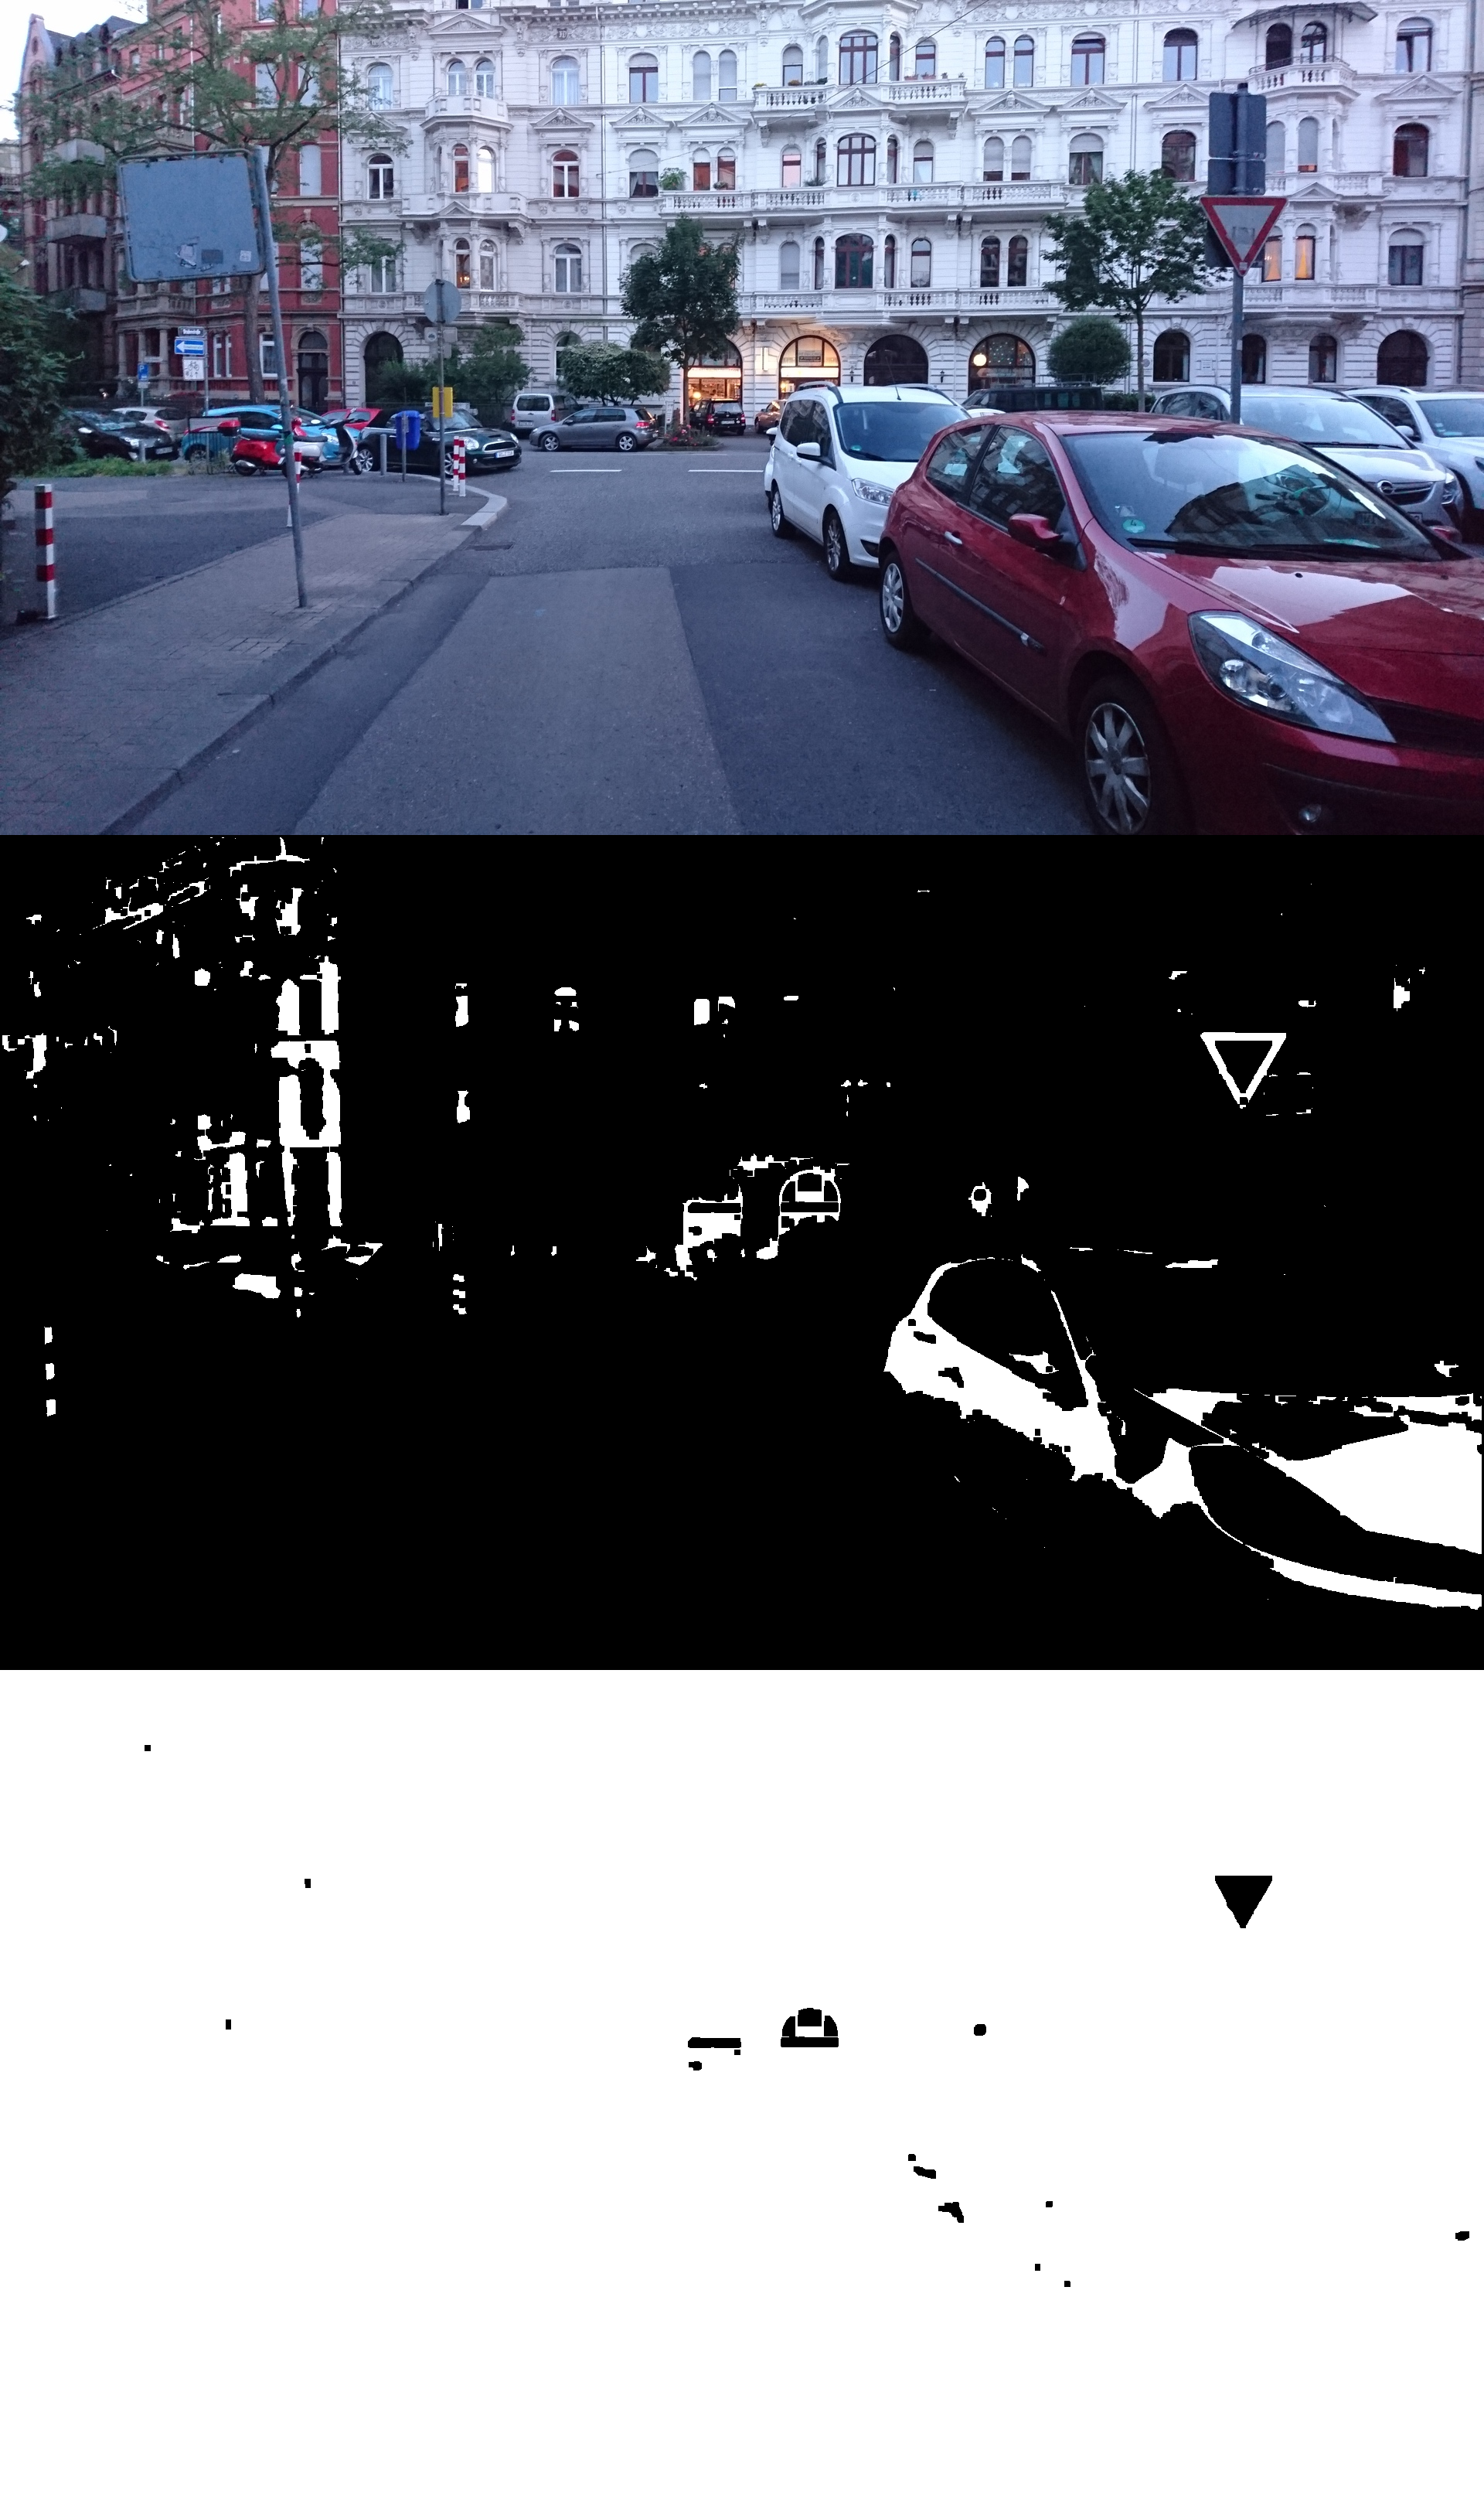
\includegraphics[width=.7\textwidth, frame]{src/comp/merged}
  \caption{This image exposes multiple problems for detection as both
    a lot of more or less red objects can be found and it was captured
    at dawn where due to the low light intensity the color variance
    diminishes. Note however that due to the filling step utilizing
    component labeling most of the interfering objects vanish. The
    middle image exhibits the state after applying segmentation and
    closing.}
  \label{img:filling}
\end{figure}


\section{Edge Detection}
\label{sec:pipeline_edgedet}
{\color{red}{To be written: Either Dilation + XOR or Sobel for Fast Hough}}


\section{Line Detection}
\label{sec:pipeline_linedet}
{\color{red}{To be written: Either Hough or Fast Hough}}


\section{Yield Sign Detection}
\label{sec:pipeline_yielddet}
{\color{red}{To be written}}


\subsection{Finding points of intersection}

The vectors returned by the hough transform contain the respective
values describing each found line by their normal vector and distance
from the images' origin. A simple method for detecting points of
intersections is to create homogeneous vectors and use their cross
product. If the third component is zero, no point of intersection is
found. Let \( A \) be a vector containing all radii and \( \Delta \)
contain all distances for \textit{n} found lines. Thus for any \( i
\in 1, \dots, n \) the homogeneous vector \( h_I \) is defined as:

\begin{equation}
  \begin{split}
    A & = (\alpha_1, \alpha_2, \dots, \alpha_n) \\
    \Delta & = (\delta_1, \delta_2, \dots, \delta_n)
  \end{split}
\end{equation}

\begin{align}\label{eq:poi}
  v_i & = \begin{pmatrix}
    sin(\alpha_i) * \delta_i \\ cos(\alpha_i) * \delta_i \\ 1
  \end{pmatrix}
  &
  w_i & = \begin{pmatrix}
    cos(\alpha_i) \\ -sin(\alpha_i) \\ 0
  \end{pmatrix} + v_i
  &
  h_i & = v_i \times w_i
\end{align}

Now all 2-permutations \( (i, j) \in \pi_2(n) \) are tried for
calculating intersections \( p_{i,j} = h_i \times h_j \). Thus the set
of all intersections is \(\{ (y, x)_{i, j} | y = \frac{p_{i, j,
    0}}{p_{i, j, 2}}, x = \frac{p_{i, j, 1}}{p_{i, j, 2}} \forall
p_{i, j, 2} \neq 0 \}\). Also, to keep all further computation small
even if a lot of lines are found, the points of intersection are
filtered by whether there is some red to be found nearby. To do so,
the result of the morphological computations (section
\ref{sec:pipeline_morph}) is consulted and the point of intersection
is kept if any white pixel is found there. An example of why this a
useful step is given in figure \ref{img:red_detection} where a
triangle is falsely classified as a yield sign although there is no
sign remotely close. The points are further filtered by whether they
are inside the image plus some boundary. Even for truncated signs the
relevant point of intersection is near the image boundary. The
parameters for controlling the size of both the lookup area and the
image boundary are free parameters. The intersections are saved as an
unambiguous mapping of \( T = min(i, j) \to max(i, j) \to (y, x)_{i,
  j} \).

\begin{wrapfigure}{r}{0.6\textwidth}
  \begin{center}
    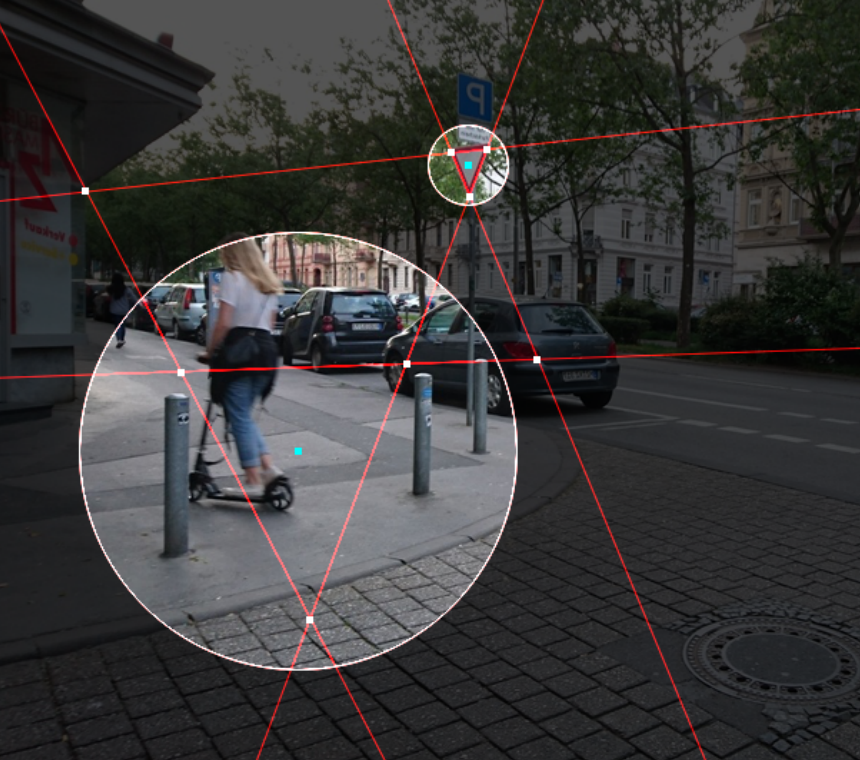
\includegraphics[width=0.58\textwidth]{src/red_detection}
  \end{center}
  \caption{An example where a triangle with the shape of a yield sign
    is found if no prior filtering of intersections based on detected
    red value is applied.}
  \label{img:red_detection}
\end{wrapfigure}


\subsection{Determining Triangles and Yield Signs}

All the previously detected candidates are now iterated by checking
whether any \( i, j, k \) exists where a combination of intersections
is transitive, meaning \( (i, j, p_0), (j, k, p_1), (i, k, p_2) \in T
\). If the condition holds, than the three points \( p_0, p_1, p_2 \)
are the vertices of a triangle and the tuple \( (i, min(j,k),
max(j,k)) \) unambiguously identifies it. Now they are filtered
further by discarding all triangles whose ratio does not fit (yield
signs are nearly equilateral, even when taking perspective into
account). Also signs can be discarded whose total size exceeds or
undercuts some threshold. These thresholds can be calculated based on
the images size.

The last step of detecting whether the found triangle actually
corresponds to a yield sign consists of looking at the actual shape of
the triangle itself. To do so, a reference triangle is created,
mimicking the shape of a yield sign, and an equally sized image with a
triangle having the shape of the detected one. Both images are binary
images where the triangles are white. Let \( ref \) be the reference
triangle image and \( tri \) the detected triangle, \( h \) the
reference images' height and \( w \) the reference images' width, then
the difference between the two is defined in
\ref{eq:detect_patmatch}. The resulting real number \( \Delta \in [0,
  1] \) expresses the similarity between the two and the larger that
value gets the more different the triangles are. Whether the triangle
is classified as a yield sign is controlled by a free parameter
threshold. This threshold can be raised to detect yield signs that are
distorted by perspective.

\begin{equation}\label{eq:detect_patmatch}
  \Delta = \frac{1}{h * w} \Bigg( \sum_{0 \leq y < h}\sum_{0 \leq x <w} ref(y, x) \oplus tri(y, x) \Bigg)
\end{equation}


\begin{figure}
  \begin{subfigure}[t]{0.3\textwidth}
    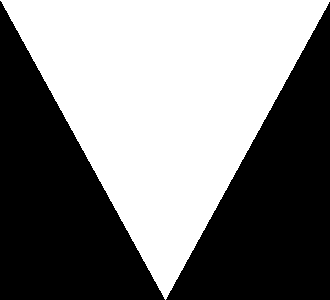
\includegraphics[width=1\textwidth]{src/patmatch_ref}
    \subcaption{\centering The reference triangle}
  \end{subfigure}
  \qquad
  \begin{subfigure}[t]{0.3\textwidth}
    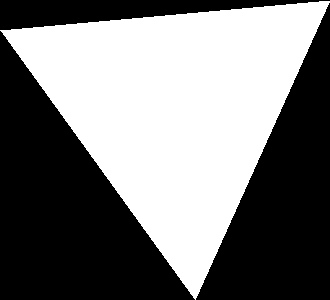
\includegraphics[width=1\textwidth]{src/patmatch_tri1}
    \subcaption{\centering Most likely a yield sign with \( \Delta \approx 0.12 \)}
  \end{subfigure}
  \qquad
  \begin{subfigure}[t]{0.3\textwidth}
    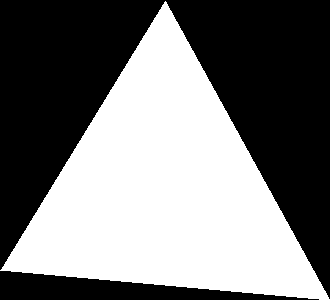
\includegraphics[width=1\textwidth]{src/patmatch_tri2}
    \subcaption{\centering This could be a warning sign with \( \Delta \approx 0.47 \)}
  \end{subfigure}
  \caption{Example results of equation \ref{eq:detect_patmatch}}
\end{figure}


\pagebreak
\chapter{Evaluation}
{\color{red}{To be written}}

\section{Performance}
{\color{red}{To be written}}

\section{Application to Videos}
{\color{red}{To be written (ROI, Frame-Skipping)}}

\section{Prospect}
{\color{red}{To be written (Other approaches: k-means clustering for
    segmentation, Otsu? ...)}}


\pagebreak
\chapter{Conclusion}


\end{document}
